Маятник Максвелла представляет собой диск, неподвижно закрепленный на тонком стержне. На концах стержня симметрично относительно диска закреплены нити, с помощью которых маятник подвешен к штативу. При вращении маятника нити могут наматываться на стержень или сматываться с него, обеспечивая тем самым перемещение маятника вверх - вниз. Если, намотав нити на ось, поднять маятник на некоторую высоту и отпустить его, то он начнет опускаться под действием силы тяжести, приобретая одновременно и вращательное движение. В нижней точке, когда маятник опустится на полную длину нитей, поступательное движение вниз прекратится. Нити станут наматываться на вращающийся по инерции стержень, а маятник начнет подниматься вверх, постепенно замедляя свое вращение. После достижения наивысшей точки цикл колебательного движения возобновится.

Делаем следующие допущения в модели: 
\begin{itemize}
\item нити невесомы; 
\item ось и диск сделаны из одинаковых материалов; 
\item нет трения о воздух; 
\item потерями кинетической энергии ввиду трения нити об ось и местах крепления пренебрежем; 
\item нить почти нерастяжима, то есть не растягивается под действием силы тяжести при обычном движении диска. Но когда нить раскручивается до конца, происходит упругий удар, и маятник теряет часть энергии, но на длине нити это не сказывается. Кстати это допущение почти не изменяет реальной картины: колебания затухают, но нить не удлиняется.
\end{itemize}

 \begin{figure} [h] 
   \center
   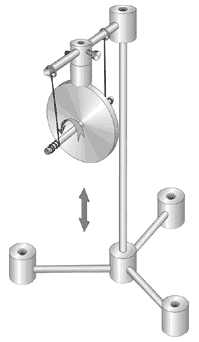
\includegraphics {HML_PendulumOfMaxwell2.png}
   \caption{Внешний вид маятника} 
   \label{img:HML_PendulumOfMaxwell2}  
 \end{figure}
 
  \begin{figure} [h] 
   \center
   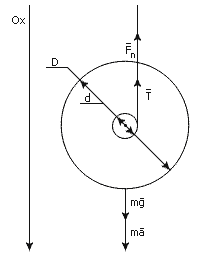
\includegraphics {HML_PendulumOfMaxwell3.png}
   \caption{Схематичное изображение} 
   \label{img:HML_PendulumOfMaxwell3}  
 \end{figure}

\textbf{Входные параметры:}
 
Data --- параметры маятника
 
 [0] --- текущее положение маятника. Сюда запишется положение маятника на  следующей итерации.
 
 [1] --- текущая скорость маятника. Сюда запишется скорость маятника на следующей итерации.
 
 [2] --- текущее значение управляющего ускорения. Если равно 0, то управления нет.
 
 [3] --- Сюда запишется значение ускорения маятника на данной итерации.
 
 [4] --- Сюда запишется, сколько на данной итерации произошло неупругих соударений.
 
 [5] --- масса диска.
 
 [6] --- масса оси.
 
 [7] --- радиус диска.
 
 [8] --- радиус оси.
 
 [9] --- длина нити.
 
 [10] --- коэффициент затухания.
 
 [11] --- интервал наблюдений.
 
 [12] --- минимальная амплитуда отскока в нижней точке. Критерий остановки.

\textbf{Возвращаемое значение:}
 
1 --- все хорошо
 
0 --- введены недопустимые данные

 \begin{figure} [h] 
   \center
   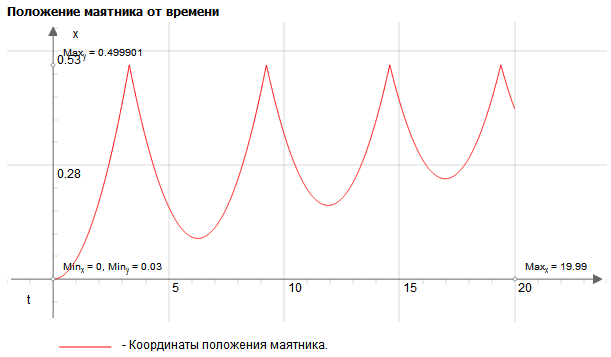
\includegraphics {HML_PendulumOfMaxwell.png}
   \caption{Пример графика координаты маятника по данной модели} 
   \label{img:HML_PendulumOfMaxwell}  
 \end{figure}